\section{Resultados}

\subsection{RTT Teórico}

En este apartado describimos el desarrollo del cálculo teórico del \textit{Roundtrip Time} (RTT).
\\
Sabemos que el RTT es el tiempo que tarda la información en ir y volver, es decir:

\begin{equation}
	Rtt = 2 * Delay
\end{equation}

Es por esto que necesitamos calcular el delay, o tiempo que tarda la información en llegar al destino desde una fuente dada:

\begin{equation}
	Delay = T_{tx} + T_{prop}
\end{equation}

Creemos acorde para este caso, considerar despreciable el tiempo de transferencia o llenado del medio $T_{tx}$, dado que en comparación al tiempo de propagación, es ínfimo. Entonces debemos calcular:

\begin{equation}
	T_{prop} = D/V
\end{equation}

con $D$ la distancia del enlace y $V$ la velocidad de propagación. La distancia del enlace varía según el caso probado, y la velocidad de propagación la sacamos del enunciado ($2*10^5$ km/s). Dados los cálculos anteriores, los resultados son los siguientes:\\

\begin{center}
\begin{tabular}{| c | c | c | c |} \hline
	Universidad		&	\textbf{Berkeley}		&	\textbf{Oxford}		&	\textbf{Tokio}		\\ \hline
	Distancia		&	10412 km		&	11107 km		&	18372 km		\\ \hline
	$T_{prop}$		&	52.06 ms	&	55.535 ms	&	91.86 ms	\\ \hline
	Delay			&	52.06 ms	&	55.535 ms	&	91.86 ms	\\ \hline
	\textbf{Roundtrip Time}	&	\textbf{104.12 ms}	&	\textbf{111.07 ms}	&	\textbf{183.72 ms}	\\ \hline
\end{tabular}
\end{center}

\subsection{RTT Empírico}

En las siguientes figuras se presentan los gráficos y diagramas realizados en función de las muestras de RTT realizadas con las distintas implementaciones de traceroute y los experimentos propuestos. Es importante aclarar que las franjas horarias mencionadas corresponden al huso horario de la ciudad origen, es decir GMT-3 según se utiliza en la Ciudad Autónoma de Buenos Aires. En caso de que la franja represente otro huso horario, la aclaración pertinente se encontrará en el análisis correspondiente al experimento. Además, en los gráficos en función de las franjas, los valores de RTT han sido promediados de un total de 20 ejecuciones de la herramienta.

\begin{figure}[h!]
  \centering
  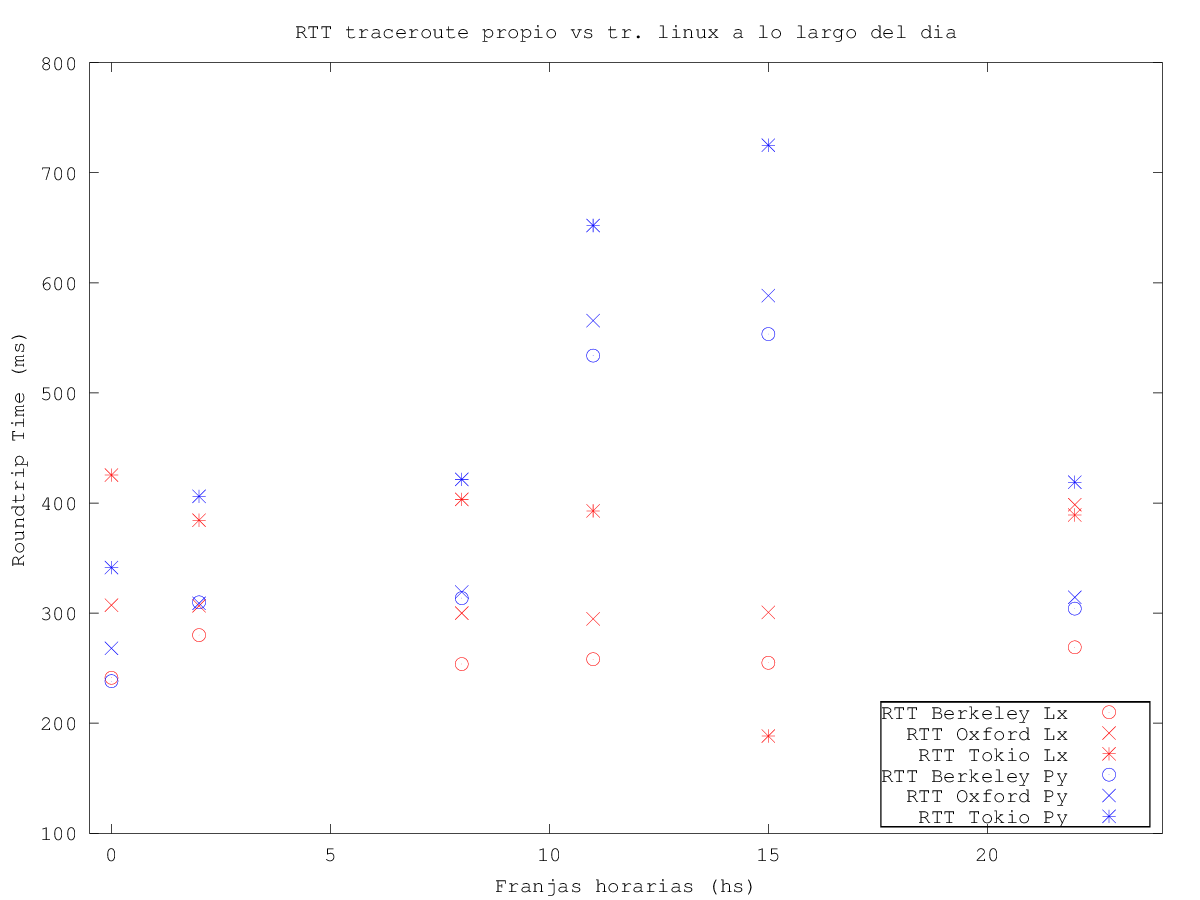
\includegraphics[width=0.6\textwidth]{./figs/franjasTR_py_vs_linux.png}
  \caption{RTTs de ambos traceroute a cada destino en función de franja horaria}
  \label{fig:frajasTR_py_lin}
\end{figure}

\clearpage

\begin{figure}[h!]
  \centering
  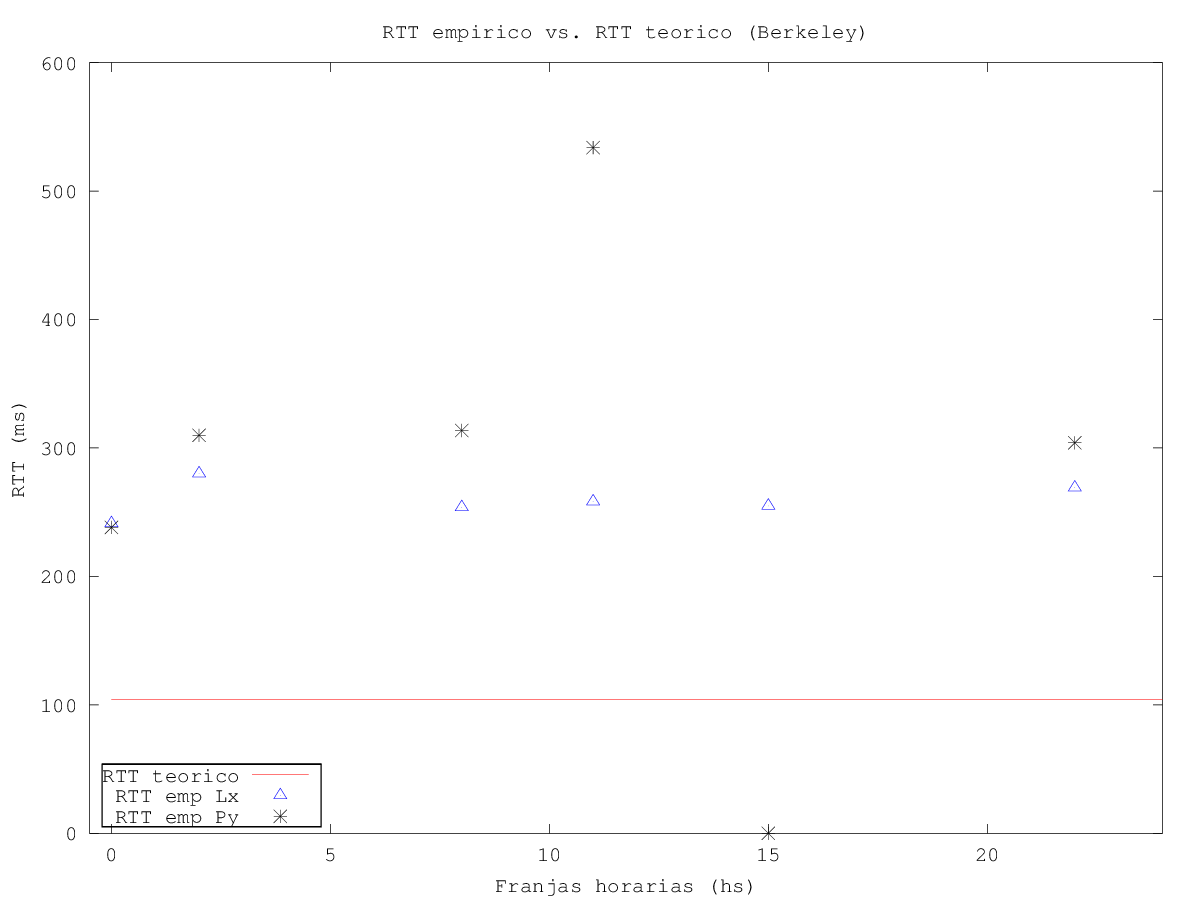
\includegraphics[width=0.7\textwidth]{./figs/rtt_emp_vs_teo_berkeley.png}
  \caption{RTTs de ambos traceroute a Berkeley en contraste con el cálculo teórico}
  \label{fig:emp_vs_teo_berk}
\end{figure}

\begin{figure}[h!]
  \centering
  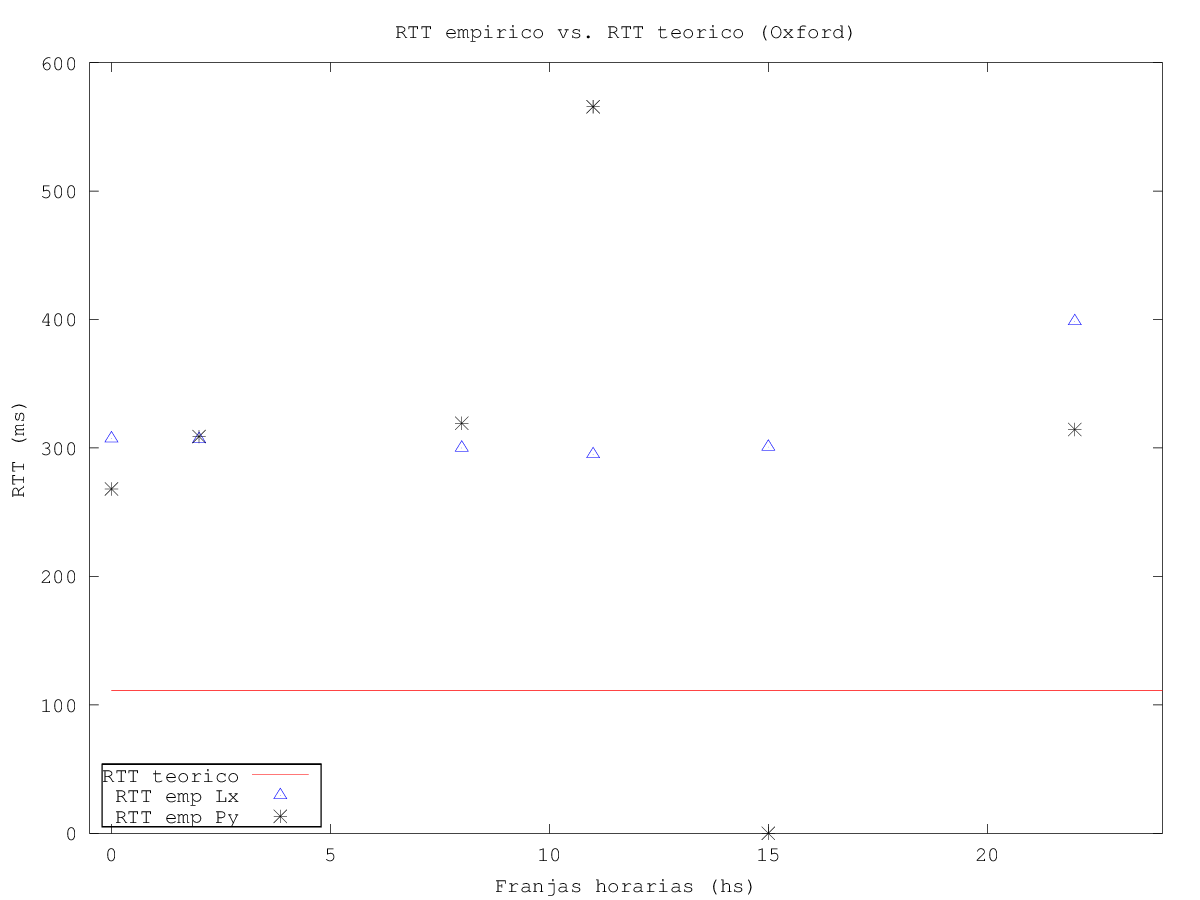
\includegraphics[width=0.7\textwidth]{./figs/rtt_emp_vs_teo_oxford.png}
  \caption{RTTs de ambos traceroute a Oxford en contraste con el cálculo teórico}
  \label{fig:emp_vs_teo_ox}
\end{figure}

\begin{figure}[h!]
  \centering
  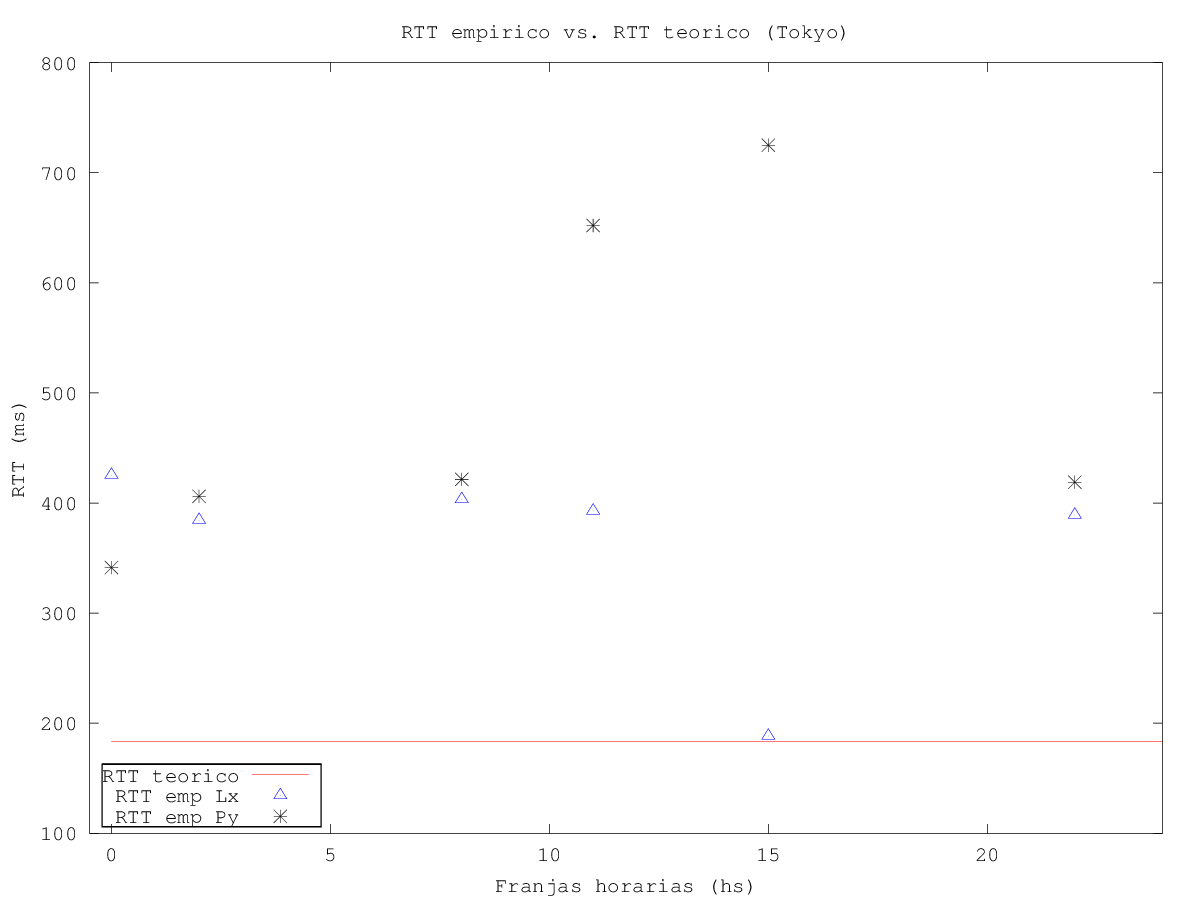
\includegraphics[width=0.7\textwidth]{./figs/rtt_emp_vs_teo_tokyo.png}
  \caption{RTTs de ambos traceroute a Tokyo en contraste con el cálculo teórico}
  \label{fig:emp_vs_teo_berk}
\end{figure}

\begin{figure}[h!]
  \centering
  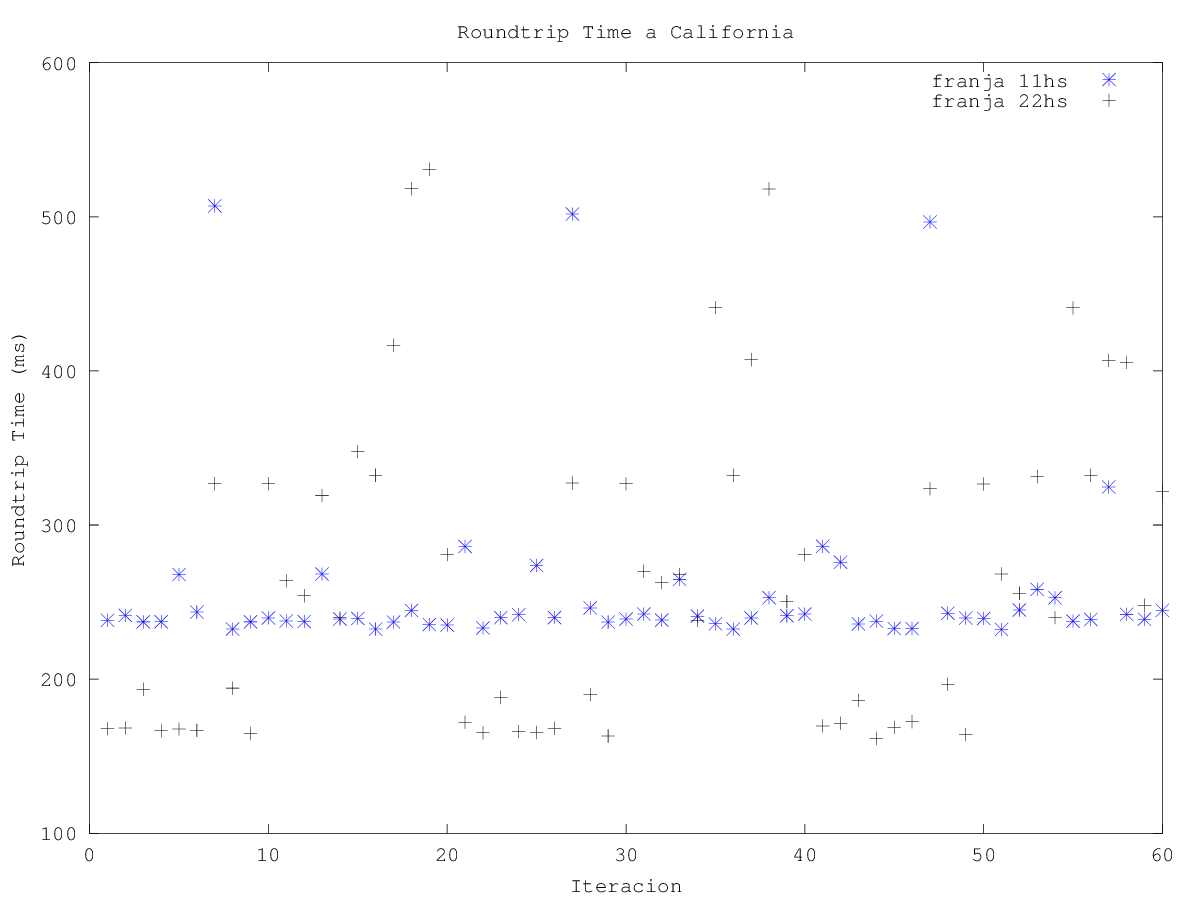
\includegraphics[width=0.7\textwidth]{./figs/rtt_horarios_california.png}
  \caption{RTT representativo de la Universidad de Berkeley, California}
  \label{fig:rtt-horarios-california}
\end{figure}

\begin{figure}[h!]
  \centering
  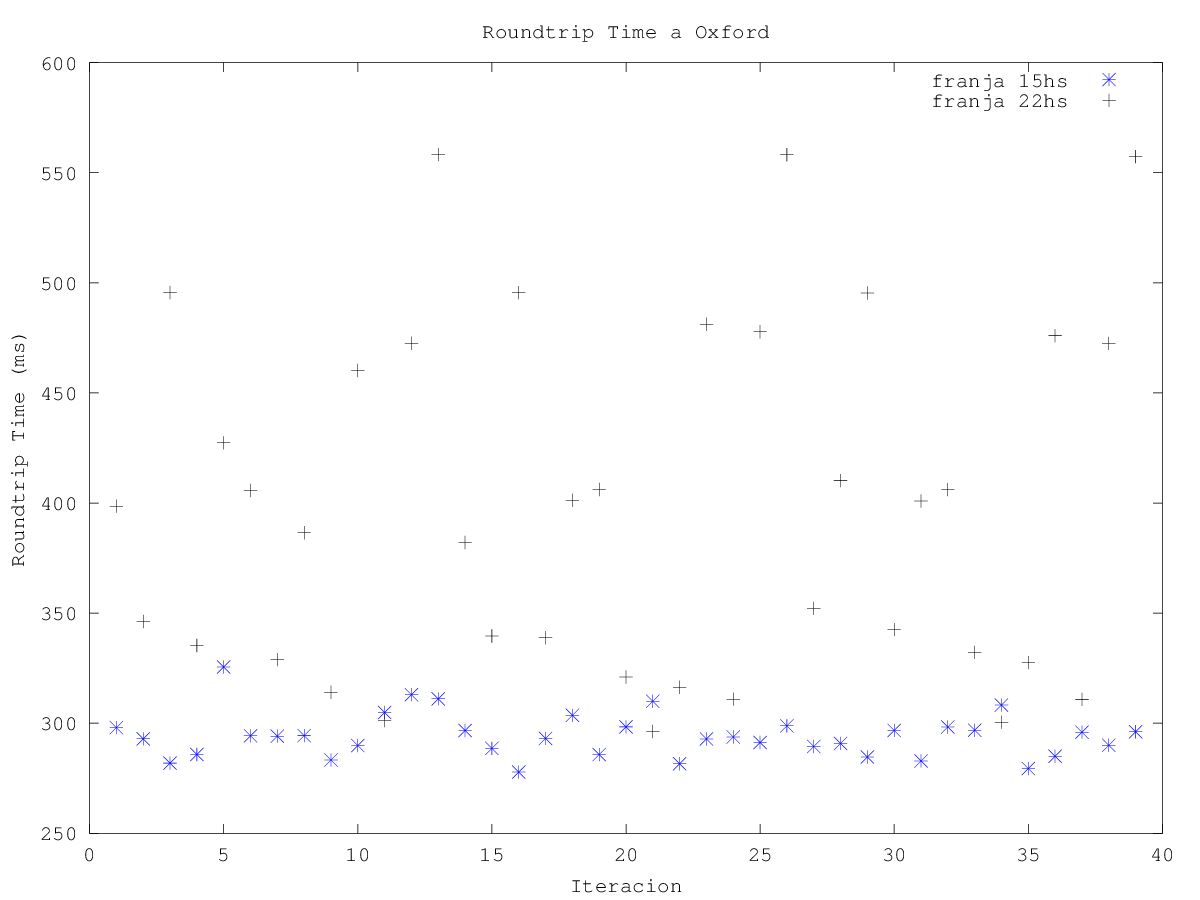
\includegraphics[width=0.7\textwidth]{./figs/rtt_horarios_oxford.png}
  \caption{RTT representativo de la Universidad de Oxford}
  \label{fig:rtt-horarios-oxford}
\end{figure}

\begin{figure}[h!]
  \centering
  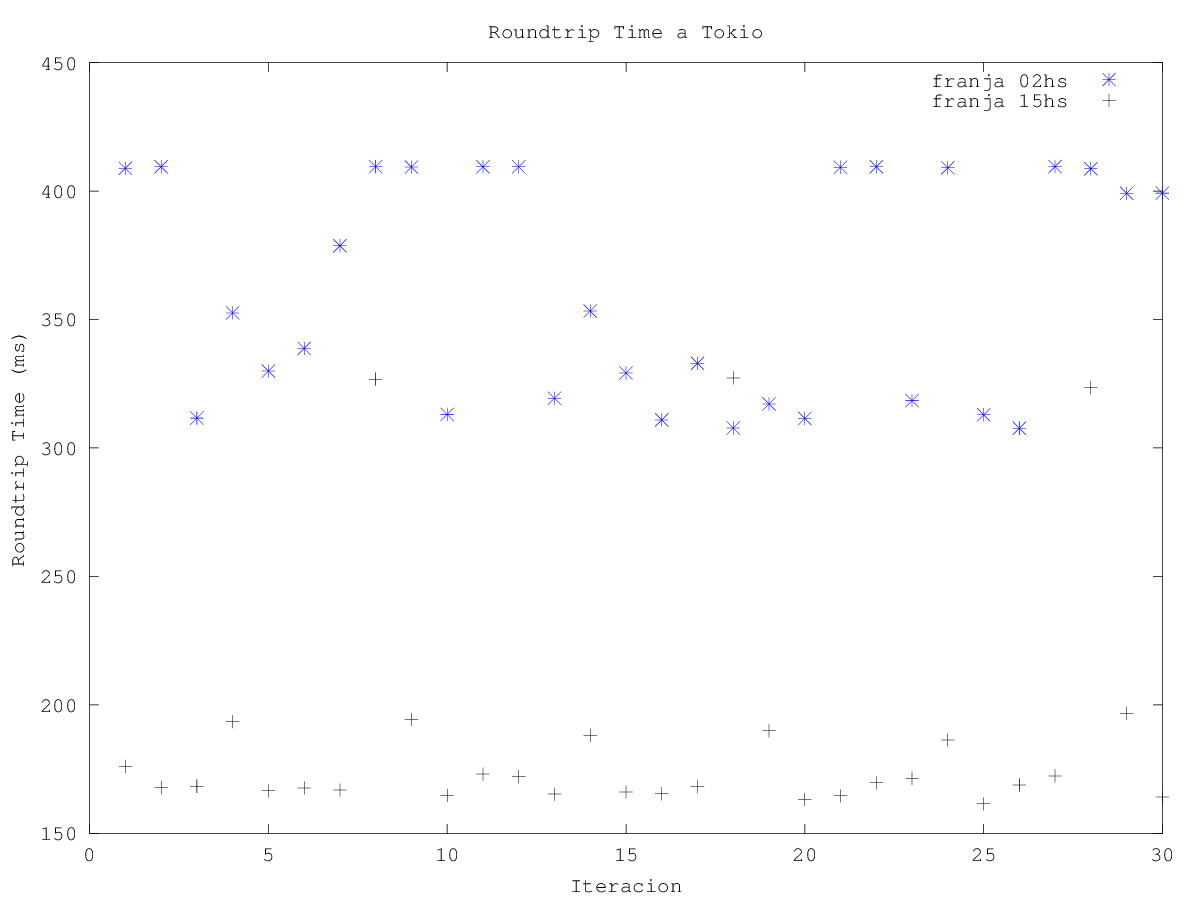
\includegraphics[width=0.7\textwidth]{./figs/rtt_horarios_tokyo.png}
  \caption{RTT representativo de la Universidad de Tokio}
  \label{fig:rtt-horarios-tokyo}
\end{figure}

\clearpage

\begin{figure}[t!]
  \centering
  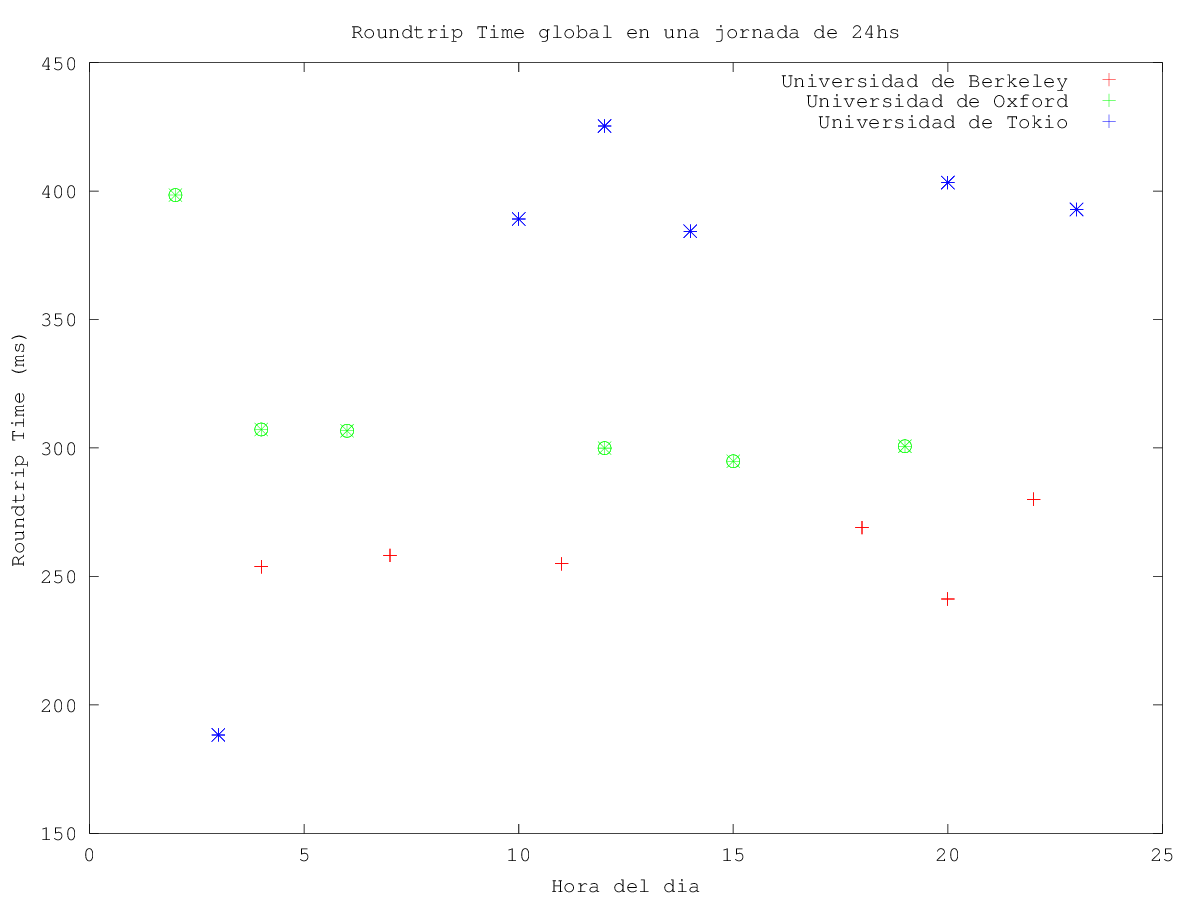
\includegraphics[width=0.7\textwidth]{./figs/rtt_normalizado.png}
  \caption{RTT a las 3 universidades en fase según un día laboral global}
  \label{fig:rtt-normalizado}
\end{figure}



